
%\subsection{Cryostat Configuration for Calibration}
%\label{sec:calib-ports}
Figure~\ref{fig:DPFDLaserPositions} shows a possible layout of the laser calibration port locations (black circles) on the cryostat roof. 

\begin{dunefigure}[Sketch of cryostat penetration map with laser calibration ports]{fig:DPFDLaserPositions}
{Top view of the \dpmod %DUNE SP FD 
cryostat showing possible laser system penetrations (black circles). The red line shows the \dword{fc} top view and the green square is one of the six \dword{crp} modules. 

}
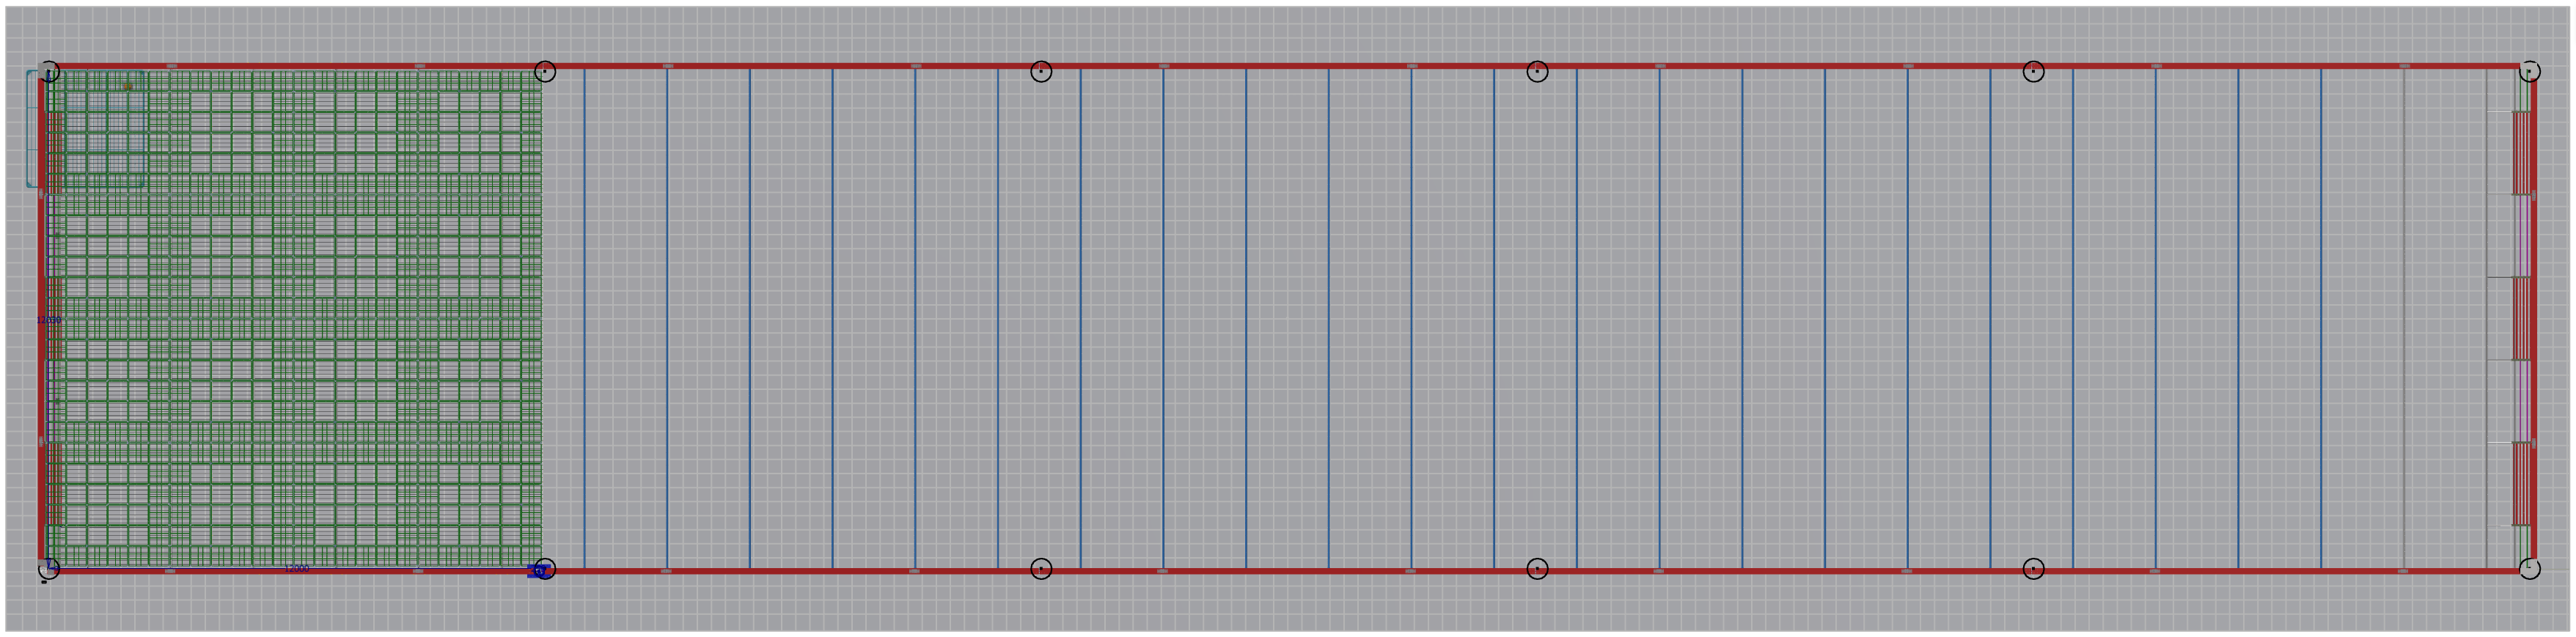
\includegraphics[width=1.0\textwidth]{DPFDLaserPositions.png}
\end{dunefigure}

The placement of these penetrations is driven by requirements of the ionization laser system and the available gaps between \dword{crp} and \dword{fc}. 
Implementing the ionization laser system as proposed in Section~\ref{sec:dp-calib-sys-las-ion} requires a total of \num{12} feedthroughs at each of the indicated ports. 

The distance between any two consecutive feedthrough columns shown in Figure~\ref{fig:DPFDLaserPositions} is approximately \SI{12}{\m}. Since the \dword{microboone} laser system has shown that tracks will propagate over that detector's full \SI{10}{\m} length, this distance is considered reasonable. Assuming that the effects of Rayleigh scattering and self-focusing (Kerr effect) do not limit the laser track length, this laser arrangement could illuminate the full volume with crossing tracks.
At this time, the maximum usable track length is unknown, and it may be that the full \SI{60}{\m} \detmodule length could be covered by the laser system after optimization.

For the \dword{pns} system, two ports, each at 1/4 of the module length (along the beam direction) from each side should be close to optimal to provide necessary coverage. The exact locations of these ports is not yet finalized.
